\begin{enumerate}[label=\thesection.\arabic*.,ref=\thesection.\theenumi]
\numberwithin{equation}{enumi}

\item
Unit Step response of a linear time invariant (LTI) system is given by 
\begin{align}
y(t) = (1 - e^{-2t})u(t)
\end{align}
Assuming zero initial condition, the transfer function of the system is

\solution We can convert this step response into s-domain using the Laplace Transform
\begin{align}
Y(s) = \mathcal{L}(y(t))
\end{align}
\begin{align}
where \quad \mathcal{L}(y(t))= \int_{-\infty}^{\infty} y(t)e^{-st} dt
\end{align}

\begin{align}
Y(s) = \mathcal{L}(y(t))
\end{align}
\begin{align}
\implies Y(s) = \mathcal{L}(u(t) - e^{-2t}u(t))
\end{align}
\begin{align}
\implies Y(s) = \mathcal{L}(u(t)) - \mathcal{L}(e^{-2t}u(t))
\end{align}
\begin{align}
\implies Y(s) = \frac{1}{s} - \frac{1}{s+2}
\end{align}
\begin{align}
\implies Y(s) = \frac{2}{s(s+2)}
\end{align}

\begin{align}
X(s) = \frac{1}{s}
\end{align}

The Transfer Function $H(s)$ is given by
\begin{align}
H(s) = \frac{Y(s)}{X(s)}
\end{align}
\begin{align}
H(s) = \frac{2}{s+2}
\end{align}
Hence the Transfer Function $H(s)$ is $\frac{2}{s+2}$\\*


\item Plot and observe the input, output and impulse response using Python
\solution
\begin{lstlisting}
codes/EE18BTECH11021.py
\end{lstlisting}

\item Comment on the stabilty of the system from the obtained transfer function

\solution
The Transfer Function is 
\begin{align}
H(s) = \frac{2}{s+2}
\end{align}
which has only 1 pole at s = -2, which is on the left half of s-plane therefore the system is stable

We can see that the output function attains a steady state of y = 1 as t tends to infinity, this is the verification that the system is stable

\begin{figure}
\centering
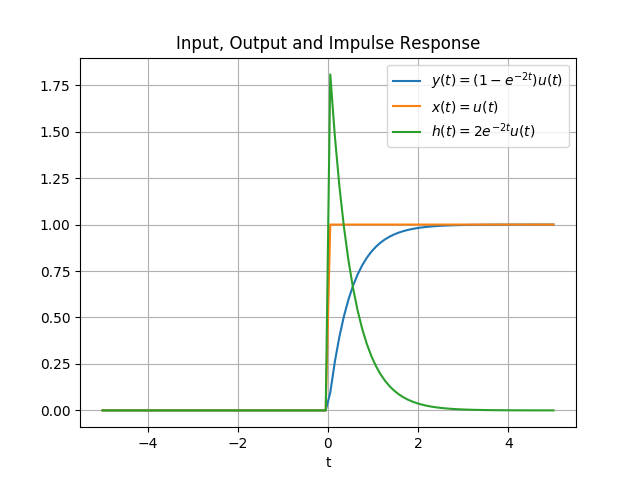
\includegraphics[width=\columnwidth]{figs/EE18BTECH11021_fig.png}
\end{figure}
\end{enumerate}
